\chapter{Discussion}
This chapter discusses and analyzes the results of the experiments, highlighting their significance in the context of the research questions. We also reflect on any limitations of the thesis and attempt to address the research questions based on the findings.

\section{Defining a baseline}

\begin{comment}
Points to discuss:
- Main point: Discuss the process of choosing which experiments was chosen.
- There might have been other experiments that should've been included in deciding the baseline.
- The way to choose which experiment goes forward could've been done differently.
- Although one experiment seem to do better with the current chosen setup, it might've done worse in another setup.
\end{comment}

In order to define a baseline for capturing data for training NeRFs, five experiments were selected and conducted: camera setup, capacity, number of frames, image size, and vehicle speed. These experiments were chosen based on heuristics and knowledge of what contributes to good NeRF results, such as well-lit scenes and non-blurry images. While the chosen experiments consider important factors for capturing data for NeRFs, there may have been other experiments that could have been included in defining the baseline. It's also important to weigh the fact that the best-performing settings in one experiment may not generalize to other setups. Overall, the process of defining a baseline is an iterative one that requires careful consideration of various factors and a willingness to continuously improve and refine the baseline.

\subsection{Camera setup}

The camera setup used in the experiment was arbitrary and may not reflect how cameras are typically rigged on cars. Future research could explore more realistic camera setups to improve the generalizability of the results. Additionally, the camera setups used in the study were sparse, with only a few cameras at specific angles. It is possible that other camera setups could yield even better results.

The results of the experiment showed relatively little difference in the quantitative metrics across the camera setups tested. However, camera setup 1 with two cameras at -10$^{\circ}$ and 10$^{\circ}$ yaw produced the highest SSIM and lowest LPIPS scores, indicating that it produced the most visually similar and perceptually pleasing images. One possible explanation of this result can be the level of overlap between the captured images the given setup provides. Both cameras have a field of view of $90^\circ$ and are mounted in the same location, resulting in a $70^\circ$ overlap between the images in the training data. This overlap means that when the model trains on an image from one of the cameras, it necessarily also trains on approximately three-quarters of the scene captured from the other camera. Because the evaluation set is a subset of the training images, it's fair to assume that the model should score high on the respective metrics.


\begin{comment}
- The position of the camera was arbitrary. Could've done more research into how cameras on cars usually are rigged.
- The camera setups are very sparse, a lot of different possibilities.

Results:
- Relatively little difference in the quantitative results.
- Why did the -10 and 10 yaw yield the best SSIM and LPIPS?
- The evaluation images are a subset of the training images. Because the -10 and 10 have a lot of overlap, they have a lot of common training data which will allow the model to learn the scene which it is evaluated on, in turn yielding high scores on the chosen metrics.


This overlap allows the model to train and learn the scene which it is evaluated on, because the evaluation set is a subset of the training images, more than the other setups, and it'll naturally score high on the respective images.

the model to train on the partial scene with two times the amount of data, and since the evaluation set is a subset of the training images, it'll naturally score high on the respective images.

\end{comment}










\subsection{Capacity} 
% Summarize the important discussion added in the experiment
As stated in the experiment's section, the longest segment was selected for the baseline despite achieving the lowest scores across the metrics. This was done to ensure that the scene encompasses a diverse range of environments, including straight roads, curves, intersections, and varying lighting conditions.

% New discussion
In the qualitative analysis of the capacity results, it's evident that the quality of the renders degrades as the segment's length increase. The most prominent deterioration is the increase in blur. A reason why PSNR remains relatively constant across the different experiments is probably in part because PSNR has been shown not to capture blur well \cite{videoprocessingai}, as exemplified by \autoref{fig:psnr-critique}. This example demonstrates the importance of evaluating the different metrics, as both SSIM and LPIPS are good metrics for capturing blur.

\begin{figure}[ht]
    \centering
    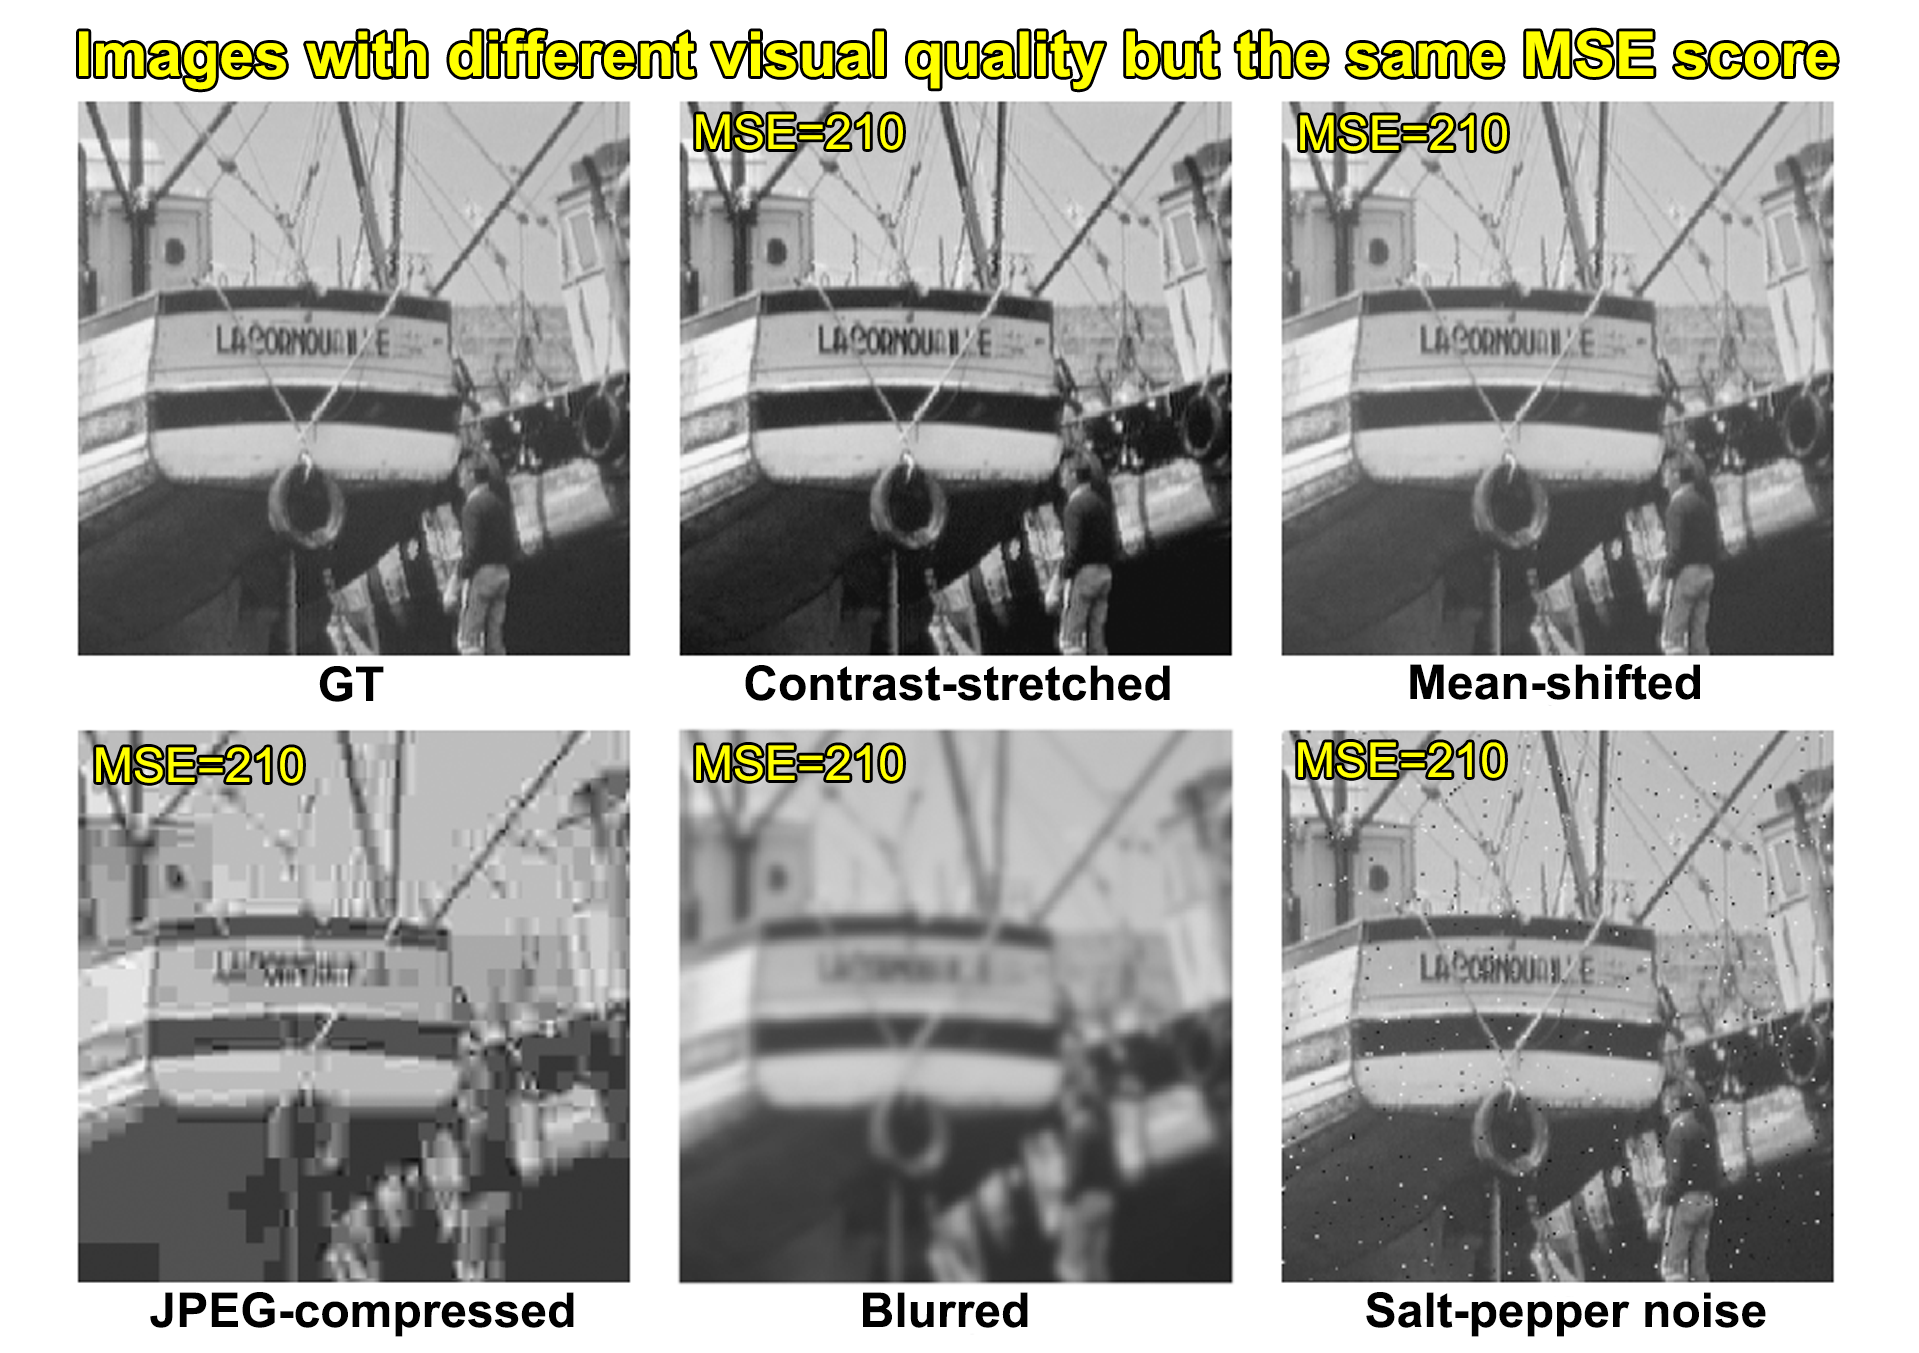
\includegraphics[width=1.0\textwidth]{figures/psnr-critique.png}
    \caption{Comparison of an image depicting a boat that has been subjected to various types of distortions.}
    \label{fig:psnr-critique}
\end{figure}

















\subsection{Number of frames}

%- The captured images are very similar
%- The default dataset size in Nerfstudio is 300 images
%- Show a mathematical proof of why more images would make sense

To comprehend the outcomes of this experiment, it would be beneficial to look into how the number of frames and the image size impact the training process. We train for 15'000 iterations where each iteration uses 4096 pixels. This results in $\sim61$ million pixels being viewed throughout a single training. With 225 images and an image resolution of $600 \times 450$, we have $\sim61$ million pixels. That means that by the end of the training, approximately all of the input pixels were trained on. A dataset containing more than 225 images and corresponding camera poses would leave abundant pixels, and any fewer would lead to pixels being trained on multiple times. This calculation would entail that the results should be relatively similar for all experiments with 1231, 615, 411, 307, and 247 images respectively. But, there is a significant drop in PSNR from experiments 1 to 4. The drop in PSNR indicates that another important factor is the variety in the dataset.


% TODO: I should discuss other options as to why the number of frames affect the metrics in the way it does.












\subsection{Image size}
Based on the metric scores, it might seem counterintuitive that the lowest resolution of $200 \times 150$ performed best. However, a deeper look at the qualitative results in \autoref{fig:image-size-comparison} reveals a different narrative. Despite lower resolutions yielding higher scores on metrics, they seem to fail in capturing fine-grained details, resulting in less visually pleasing images. On the other hand, higher-resolution images allow the NeRF model to capture and replicate more intricate details, leading to superior visual outcomes, albeit with lower metric scores. This difference can be attributed to the higher sensitivity of metrics to minor discrepancies and noise in high-resolution images, potentially causing significant metric score reductions despite only minimal perceptual differences.

Given these considerations, the chosen resolution of $400 \times 300$ for the following experiments is a balanced choice, considering both the metrics and the perceptual image quality. Furthermore, it aligns well with the chosen number of frames from the previous experiment, as the combined configuration will allow training to cover about 84\% of the input pixels.

\begin{comment}
The qualitative assessment shows clear evidence of higher resolution images leading to higher fidelity renders, although the metrics suggest otherwise. When using lower-resolution images, the metrics may become less sensitive because they are less affected by small differences between the synthesized and ground-truth images. This is because lower-resolution images have fewer pixels, which can make the metrics less precise in measuring the perceptual similarity between the images. However, using lower-resolution images can also lead to a loss of detail and fidelity in the synthesized images. When comparing low-resolution images with high-resolution images, these metrics may become less effective because the high-resolution images are more sensitive to small differences between the synthesized and ground-truth images. In other words, the NeRF may generate high-quality images that are perceptually similar to the ground-truth images, but small differences in the pixel values or noise can cause a significant decrease in the metric scores.

The chosen resolution of $400 \times 300$ aligns well with the chosen number of frames from the previous experiment. With 2 ticks per image, $\sim615$ images for the baseline, we have $\sim73$ million pixels. The training will cover about 84\% of the input pixels.

This might be a special case for synthetic data where we have perfect camera poses. With higher-resolution images, the requirement for accurate camera poses increases as the camera poses have to be aligned pixel perfect with the image.
\end{comment}












\subsection{Vehicle speed}
The reason why the faster runs achieve worse results might be attributed to the motion blur and temporal artifacts that can occur when the vehicle is moving fast. In CARLA these effects are added as part of the post-processing of the captured camera image. At higher speeds, the motion of the vehicle can cause blurring and distortion in the captured images, which can reduce the quality of the data and make it more difficult for the NeRF to learn the underlying 3D scene structure and appearance. In contrast, slower vehicle speeds can reduce the amount of motion blur and temporal artifacts, resulting in clearer and more detailed images. Another side effect of driving slower is that it leads to an increased amount of images captured. At 50\% speed, the dataset consists of 1095 images, in contrast to the 429 images captured at 200\% speed.


% The reason for this can be attributed to the motion blur and temporal artifacts that can occur when the vehicle is moving too fast. At higher speeds, the motion of the vehicle can cause blurring and distortion in the captured images, which can reduce the quality of the data and make it more difficult for the NeRF to learn the underlying 3D scene structure and appearance. In contrast, slower vehicle speeds can reduce the amount of motion blur and temporal artifacts, resulting in clearer and more detailed images. Another side effect of driving slower is that it leads to increased amount of images captured. At 50\% speed, the dataset consists of 351 images, in contrast to the 131 images captured at 200\% speed.
























\subsection{Combined baseline}
% I might not need the initial "Defining a baseline" if I sum it up in this chapter.
\begin{description}[leftmargin=!,labelwidth=\widthof{RQ 1:}]
\item[\textbf{RQ 1:}] What are the critical factors that need to be considered when capturing synthetic data for training NeRF models, and how do they impact the performance of the resulting models?
\end{description}


From the experiments discussed above, it's evident that they all contribute to the quality of the data capture, which in turn contributed to the quality of the image synthesis from the resulting NeRF. Nevertheless, it is challenging to quantify the extent to which each of the different configurations affects the quality of the final baseline results.

Looking at the experiments separately, image resolution had the largest span between the quantitatively best and worst metrics. Nevertheless, the qualitative results indicated that the quantitative comparison didn't convey a fair comparison of the render-quality. Due to this, the capacity-experiment could be the experiment with the most impact on the final result.

In conclusion, when capturing synthetic data for training NeRF models, it's important to consider the camera setup, segment length or scene size, dataset size, image size, and vehicle speed. Each of these parameters presents unique influences on the quality of the data captured, and in turn, the performance of the resulting NeRF models.


\begin{comment}
The critical factors that must be considered when capturing synthetic data for training NeRF models, as inferred from the discussed baseline experiments, encompass camera setup, capacity, number of frames, image size, and vehicle speed. Each of these factors demonstrates a unique impact on the performance of the resulting models.

Camera setup plays a significant role in determining the quality of data captured for NeRF models. The experiments revealed that certain camera arrangements, specifically a setup with two cameras at -10$^{\circ}$ and 10$^{\circ}$ yaw, can result in superior SSIM and LPIPS scores, indicating more visually similar and perceptually pleasing images. This finding can be attributed to the degree of overlap between images captured by each camera in the setup. However, the experiments also highlight that camera arrangements were arbitrary and future research may investigate more realistic setups to better generalize the results.

The capacity, or the length of the road segment covered, also impacts the performance of the NeRF models. Even though longer segments led to lower scores across the metrics, these were still selected as the baseline to ensure a diverse range of environmental exposure for the model. It was noticed that the quality of renders deteriorated, especially in terms of increased blur, as segment length increased. Hence, the capacity of data has implications on the clarity and diversity of the training set, which could potentially influence the robustness of the model to diverse scenarios.

The number of frames in the dataset is another crucial factor. An optimal balance between the number of images and the image resolution is important for efficient training. In the experiments, a dataset with 225 images, each with a resolution of $600 \times 450$, covered approximately all of the input pixels by the end of training. However, a dataset with too many or too few images could result in either underutilization or overutilization of the pixels during training. Additionally, a decrease in PSNR with a drop in the number of frames points to the role of variety in the dataset.

The size of the images, or their resolution, has a complex impact on model performance. While higher resolution images contribute to higher fidelity renders, the metrics could suggest otherwise due to their increased sensitivity to minor differences in synthesized and ground-truth images. Hence, resolution can impact the quality of synthesized images and their metric scores, and it is crucial to align it with the number of frames for efficient coverage of input pixels.

Vehicle speed is a significant factor when capturing synthetic data, particularly due to the influence of motion blur and temporal artifacts on image quality. Faster vehicle speeds can lead to increased blur and distortion, making it challenging for the NeRF to learn the scene structure and appearance. Conversely, slower speeds provide clearer and more detailed images, improving the quality of the training data. Furthermore, slower speeds result in a larger dataset due to the increased number of images captured.

In conclusion, each of these factors—camera setup, capacity, number of frames, image size, and vehicle speed—has a unique and important influence on the quality of synthetic data captured for training NeRF models. Their careful consideration is essential for optimizing the performance of the resulting models.
\end{comment}








\section{Adding noise}
\begin{description}[leftmargin=!,labelwidth=\widthof{RQ 1:}]
\item[\textbf{RQ 2:}] How does the accuracy of initial camera poses and segment size influence the effectiveness of camera pose optimization, and is it possible to achieve equivalent results by optimizing rough camera poses directly, as opposed to pre-processing an approximation of accurate camera poses with tools such as COLMAP?
\end{description}

This research question addresses the effects of imperfect camera poses, frequently encountered in real-world scenarios due to GPS/GNSS inaccuracies, on the performance of camera pose optimization. We examine this by adding Gaussian noise to camera poses obtained from the CARLA pipeline, simulating real-world errors in the accuracy of these poses.

Despite Gaussian noise not perfectly replicating real-world noise distributions, its application allows a meaningful examination of camera pose optimization within our Nerfacto-pipeline. It is noteworthy that while the quantitative distinction between the non-optimized and optimized camera pose results might appear marginal, the qualitative contrasts outlined in both \autoref{fig:noise-short-segments} and \autoref{fig:noise-baseline-segments} deliver strong evidence of the camera pose optimization's effectiveness.

Particularly, the qualitative comparison highlights that the optimized camera poses generate consistently higher quality renders, even under significant noise levels. This is more discernible within shorter segments, where the optimization seems more efficient than in larger baseline scenes. This finding may be attributed to the previously discussed limitations in capacity, given that the camera optimization treats camera pose parameters as jointly optimized learnable parameters along with the RGB values.

Interestingly, the only instance where non-optimized poses yield superior results is when no noise is introduced. In such cases, the resulting render from non-optimized camera poses appears considerably sharper than its optimized counterpart, which may appear somewhat blurred. However, this outcome is most likely unique to synthetic datasets with perfect camera poses.


When examining the effectiveness of COLMAP pre-processing against the joint optimization of initial camera poses along with the other learnable parameters, it becomes evident that COLMAP tends to deliver superior performance. This observation holds particularly when the initial rough camera poses are influenced by a rather minor noise adhering to a Gaussian distribution with a standard deviation of $0.1^2$. Under these conditions, all three key metrics (PSNR, SSIM, LPIPS) associated with the NeRF lag behind those achieved by COLMAP, as can be seen from \autoref{tab:colmap-vs-poses} and \autoref{tab:exp-gaussian-noise}. Furthermore, when the noise's standard deviation is escalated to $0.5^2$, which is fair to assume could occur during real-world data capture, the metrics degrade even more significant compared to what COLMAP can deliver. While the processing time required by COLMAP might seem prohibitively lengthy for large datasets, this concern can be addressed by splitting the data into smaller sections. Thus, despite the initial time investment, COLMAP's superior performance merits consideration, particularly in scenarios with significant noise in initial camera poses.

\begin{comment}
The horizontal and vertical vectors in each experiment are subject to equal Gaussian noise. This approach may not fully capture the variability in noise that arises from realistic data capture scenarios, where factors such as the direction and speed of the vehicle can affect noise distribution. Nevertheless, the use of Gaussian noise enables the evaluation of the impact of camera optimization in the Nerfacto-pipeline.

While the difference in quantitative results between the runs with- and without camera pose optimization appear small, the qualitative comparison depicted in both \autoref{fig:noise-short-segments} and \autoref{fig:noise-baseline-segments} provides compelling evidence of its efficacy. Contrary to the NeRF that doesn't optimize the camera poses, the renders from the NeRF that optimized the camera poses remain relatively high-quality even when there is a substantial amount of noise added. This is particularly noticeable on shorter segments, where the optimization appears to perform even better than on the larger baseline scene. The observation can likely be ascribed to the capacity limitations previously discussed. This is because the camera optimization approach treats the camera pose parameters as learnable parameters that are jointly optimized with the RGB values.

The only scenario where NeRF with non-optimized camera poses outperforms its optimized counterpart is when no noise is added. In such cases, the resulting render is notably sharper than that produced by the optimized NeRF, which can appear more blurred. This finding is likely exclusive to synthetic datasets with perfect camera poses.
\end{comment}


\begin{comment}
DON'T NEED THIS SECTION BECAUSE THE COLMAP-RESULTS ARE DISCUSSED IN COMBINATION WITH THE NOISE-EXPERIMENT ABOVE.

\section{COLMAP vs. Absolute poses}
From the quantitative results, it appears COLMAP optimizes the camera poses similar to the camera pose optimization step in the Nerfacto-pipeline. When we turn off the camera pose optimization step, the perfect poses from CARLA enable even higher scores across the metrics and sharper renders.
\end{comment}





\section{Different models}
\begin{description}[leftmargin=!,labelwidth=\widthof{RQ 1:}]
\item[\textbf{RQ 3:}] How do different NeRF methods (mip-NeRF, instant-ngp, Nerfacto, Nerfacto-big) perform on unbounded scenes in terms of reconstruction quality and computational efficiency?
\end{description}

Upon examination of the different NeRF methods, namely Nerfacto, Instant-ngp, Nerfacto-big, and mip-NeRF, it is evident that their performance in terms of reconstruction quality and computational efficiency on unbounded scenes exhibits some noteworthy distinctions. Despite the differences, some of the methods demonstrate rather comparable metrics. 

Both Nerfacto and Instant-ngp demonstrate high performance on the evaluated metrics, showcasing their proficient ability to effectively learn and represent the unbounded scene. The largest deviation between the two models is their LPIPS score, where Nerfacto outperforms Instant-ngp. Nerfacto-big is a differently configured Nerfacto-model featuring an expanded hidden layer width, increasing the model's capacity. Despite being trained for a significantly larger number of iterations it fails to exceed the performance of its less complex counterparts.

Mip-NeRF, which is designed for bounded scenes, predictably falls short in learning the unbounded scene. It yields the lowest scores across all metrics. The qualitative evaluation further support this, showing no perceivable scene structure in its renderings, despite producing some correct color representations.

Given these findings, Nerfacto emerges as a strong candidate for subsequent experiments. Further more, it should serve well as a backbone-model for applications to build upon, thanks to its balance between reconstruction quality and computational efficiency.





\section{Block NeRF}
\begin{description}[leftmargin=!,labelwidth=\widthof{RQ 1:}]
\item[\textbf{RQ 4:}] What are the technical challenges and considerations for implementing a functional approach for large-scale NeRF within the Nerfstudio API, and how does it compare to approaches not optimized for large-scale in terms of scalability, efficiency, and rendering quality?
\end{description}

Implementing a functional approach for large-scale NeRF within the Nerfstudio API has been technically challenging, as elaborated upon in \autoref{sec:method-block-nerf}. However, the initial naive Block NeRF approach has displayed encouraging performance in both quantitative and qualitative aspects. The experimental results confirm that compared to training single NeRFs on large scenes, the Block NeRF approach yields superior outcomes. The image synthesis produced by the Block NeRF approach exhibits sharper details and an overall enhancement in the visual quality.

While the naive implementation of Block NeRF doesn't inherently exhibit optimal scalability, it holds significant potential for improvement. In its current state, each Block NeRF is trained sequentially, creating a bottleneck that limits scalability. However, the architecture provides an opportunity for horizontal scaling, which could be achieved by parallelizing the unique training processes across multiple GPUs. This adjustment would drastically improve efficiency and reduce training time, thereby enhancing scalability.

Nevertheless, it's important to acknowledge that this process is computationally intensive, and care should be taken to find a balance between the quality of the results and the efficiency of the process. Future work could focus on optimizing this balance to make large-scale NeRF more viable and efficient, while maintaining the high-quality image synthesis that the Block NeRF approach has demonstrated thus far.





\subsection{Improving Block NeRF}
%The overlap between the blocks become substantially less visible with higher overlap values, $\delta$. When we increase $\delta$, we increase the dataset of each block leading to the capacity issue previously explored. In a production setting, it'll be important to tune all these parameters to effectively maximize quality across all blocks.

While our approach of incorporating overlap between the Block NeRF's data resolves the problem of visible artifacts during the transition between Blocks, it is evident from \autoref{fig:block-nerf-frame-comparison} that the final frame of a block produces renders of lower quality compared to the initial frame of the subsequent block. This is to be expected if the second block's data has been captured near the respective motive seen from both blocks. This difference could probably be further mitigated by experimenting with image-merging techniques, e.g. by rendering the view from both blocks and merging them with inverse distance weighing.

%Further improvements that could be done:
%- The details of the scenery in the second frame is clearly better than the first, which is expected as block number 2 has been trained on close-up images of the scene. This difference could be mitigated by looking into image-merging techniques such as inverse distance weighing.



\section{Real data}
The naive Block NeRF approach emerges as the clear frontrunner in our experiments on real data, producing both the best quantitative and qualitative results. This finding aligns with expectations considering the scale of the scene being learned, which potentially surpasses the capacity of a single NeRF. Among all conducted experiments, the Block-NeRF run, with camera poses approximated by COLMAP without further optimization, demonstrated a distinct supremacy across all metrics, affirming the advantage of COLMAP-based pose estimation over GPS-derived alternatives.

In the subset of experiments excluding the naive Block-NeRF approach, the approach utilizing COLMAP without subsequent optimization yielded the best results. Among the runs with camera poses estimated from GPS-readings, those involving subsequent camera pose optimization produced superior metrics. These findings further support the observation that camera poses that are near-perfect tend to be disadvantaged by subsequent optimization, while imperfect camera poses benefit from this process. This observation is further reinforced by the qualitative evaluation of the different runs, presented in \autoref{fig:trip086-comparison}, where the output from runs utilizing near-perfect camera poses tended to exhibit blurriness upon subsequent optimization. In contrast, the use of subsequent optimization of imperfect camera poses enabled the NeRF to generate more precise and clear renderings.



\begin{comment}
% Discuss the implementation of rotation matrix
- The estimation could be further improved by investigating techniques for leveraging more of the contained data.
- The NAPLab car's accelerometer could be used to calculate roll and pitch.
- LiDAR data could be used for further pose estimation
\end{comment}





\section{Novel views along altered trajectory}
One of the benefits of using NeRFs in autonomous vehicle training is the ability to generate data along altered trajectories. While this can be achieved with a simulator, as discussed in \autoref{sec:wayve}, the application of NeRF becomes particularly useful when a high-quality NeRF has been trained on real data. In addition to evaluating the autonomous agent in a novel environment, the NeRF can be used to expand the training dataset for the autonomous vehicle by creating an arbitrary number of altered camera paths and synthesizing photo-realistic novel views of altered trajectories. This can help improve the robustness and generalizability of the autonomous agent by exposing it to a wider range of scenarios and viewpoints.

Looking into the experimental results from \autoref{sec:altered-trajectories}, it's important to note that the absence of ground truth images from the altered path inherently constrains our ability to conduct quantitative analysis beyond the initial evaluations. The qualitative assessment is thus the primary mode of evaluation. From the renderings depicted in \autoref{fig:altered-trajectories}, we can clearly see the potential of this application. Although the novel-rendered perspectives do not always match the quality and coherence found in the original evaluation images, they are largely successful in producing clear and structurally accurate visualizations. This affirms their potential and the effectiveness of the approach.



\section{Shortcomings}
Several areas of potential improvement can be recognized within this study. Firstly, while our research has illuminated key aspects of data capture, the time constraints of the project did not allow us to validate these findings through real-world testing. Synthetic data sets were leveraged extensively and provided evidence that the combined configurations for the baseline were promising. However, the validity of these results has yet to be confirmed on real data.

Secondly, there exist limitations in the capture of real data, specifically in the estimation of transformation matrices. The camera poses' translational components are derived from raw GNSS-readings, and the rotational components are estimated through trigonometric comparisons of adjacent GNSS-readings. Such a method is inherently susceptible to errors and inaccuracies. To improve the accuracy and reliability of data capture, a better approach could be to utilize both of the vehicle's GNSS sensors and integrate the vehicle's accelerometer data to achieve precise roll and pitch estimations.

These identified limitations present potential avenues for further research and improvement, offering opportunities to refine and enhance the existing methodology and outcomes of the study.